\chapter{Discussion}
\label{discussion}
% \begin{itemize}
%     \item The failure to collect many stripped functions is caused by decompilation issues, particularly a failure of Ghidra to align the functions, without the symbol table this is difficult
%     \item Deduplication lowers performance, but for the decompiled and demi-stripped the model is still very much usable. Duplicates are a part of the problem space.
%     \item We find that the loss of identifiers significantly lowers the performance of the model, but stripped code also suffers from decompilation faults, which have a large impact on the model performance
%     \item From the pre-training objectives, the DOBF objective is the one that worked best and the only one that did better than the base model. This is likely because the output is most like NL compared to other objectives, other objectives weaken the decoder by making it predict PL
%     \item From manual observation, we can see that the stripped decompiled code is very weakly decompiled, with few recovered identifiers, we use a relatively strong stripper, which makes the task inherently harder.
% \end{itemize}
% \newpage
In this chapter, we will provide an analysis and reflection on the results of the experiments. Furthermore, we will discuss the threats to validity and the implications of this work.

We found a relatively large difference between the number of recovered decompiled and stripped decompiled functions. This can likely be attributed to the fact that Ghidra struggles a lot more with recovering stripped functions. Recall that the symbol table commonly contains information regarding the location and name of functions. When this table is dropped, the start- and endpoints of functions are hard to infer by automatic tools, especially since many functions get inlined, and \(JUMP\) instructions replace \(CALL\) instructions. Asides from difficulties in demarcating functions, it is also difficult to align the associated source code function with the decompiled function. With unstripped code, the function name remains, meaning the functions can be aligned using the name. We attempted to utilize an existing solution by~\citeauthor{FunctionBoundaryDetection} called Jima~\cite{FunctionBoundaryDetection} to find function boundaries. Jima is the current SOTA tool for function boundary detection in stripped binaries. The tool is implemented as a plugin for Ghidra, but in our experiments, we find no statistical difference between the base performance of Ghidra and Jima on our own dataset.

The model produced many instances where the output was grammatically correct and resembled an accurate summary but is meaningless in the context of the targeted function. This shows that the model, or more specifically the decoder, knows the output language well. This is likely because of the pre-training, which included several natural language objectives, and the fine-tuning, which is exclusively focused on natural language.

Duplicates have a relatively significant impact on performance. Removing duplicates from the dataset puts the model's performance more in line with other deduplicated datasets, such as the CodeXGlue dataset used for CodeT5. Removing duplicates has a more considerable impact on decompiled code than on source code. As noted previously, duplicates are part of the problem space. We, therefore, consider them in the other experiments.

We find a relatively small difference in performance between source code and decompiled code. This indicates that in-function-comments and variable names are relatively unimportant for the model performance. Although ~\citeauthor{PolyglotCodeBERT} observed that identifiers might be more important than syntax in the code-summarisation task, we can further conclude that the function name is explicitly essential for model performance. Removing the function name from the decompiled samples, as opposed to removing all identifiers in demi-stripping, results in slightly higher performance than demi-stripped code, which indicates a very high dependence on the name of the function in the code-summarisation task. 

The prediction of function names from the function body is an already defined task, called "extreme summarisation", discussed in Chapter \ref{background}. While extreme summarisation will help recover function names for stripped functions, which can aid understanding, it has limited applicability to unstripped code, which still retains its function names. In Appendix \ref{app:ExtremeSum} we report on a few experiments on this task. We find that, similar to the regular summarisation task, and the model struggles with stripped code due to compiler issues, so we decided not to pursue this avenue any further. 

Stripped code performs significantly worse than the demi-stripped code, even when the dataset size is matched. This indicates that the decompilation failures, which occur more with stripped code, also greatly impact model performance.

Our choice of stripper might also influence the performance of the model. We find that our stripped code does not benefit from Ghidra's decompiler as much as other examples. For example, the decompiled stripped binaries used by \citeauthor{Nero} contain much more details than our samples. The sample shown in figure \ref{fig:Nero} is a binary compiled using GCC and optimisation level zero.

\begin{figure}[!h]
  \centering
  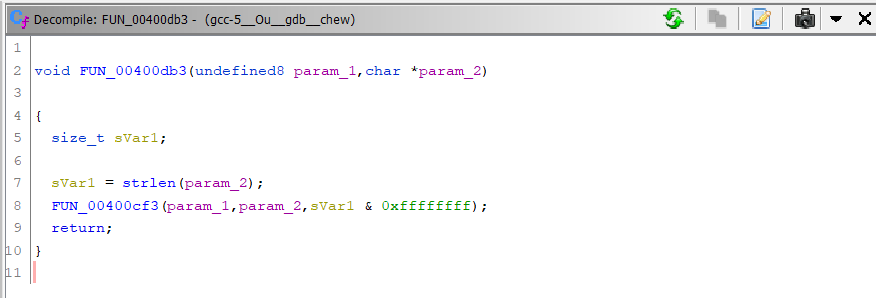
\includegraphics[width=\linewidth]{img/Nero.png}
  \caption{Short decompiled function from the GNU Debugger~\cite{Nero} decompiled by Ghidra}
  \label{fig:Nero}
\end{figure}

We observe that Ghidra's decompiler manages to recover a variable name and an external call to the strlen function. However, in our stripped samples, we do not observe this behaviour, none of the library functions is recovered, and Ghidra predicts no variable names even in samples compiled using -O0.

From the intermediate-training objectives, we find that the translation task lowers performance. There could be two explanations for this: Firstly, the model is intermediately-trained on a PL-to-PL objective, while the fine-tuning objective is a PL-to-NL objective. This causes a so-called mismatch in training objectives. Recall that Transformers \ref{background} encodes the input into embedding space using an encoder. The decoder will then transform this embedding into the output. In this case, this mismatch in objectives causes the decoder to be weakened in PL-to-NL tasks by the intermediate-training objective. During the pre-training phase, which is applied by~\citeauthor{CodeT5}, the objectives are a mix of NL-to-PL, PL-to-PL and PL-to-NL tasks. This allows a single model to be flexible and to be applied to different tasks.

The second explanation for the lower performance after TRANS intermediate-training is that the target length is also different. While the output for code summarisation is at most 12 tokens long, Neural Code Translation has a target length of 512 tokens. In general, longer target sequences make it difficult for the Transformer model to apply the attention gradient over the entire sequence length properly.

The DOBF and SPAN intermediate-training objectives do yield better performance. Both of these objectives solve the objective mismatch issue and are PL-to-NL objectives. The DOBF performed slightly higher, which could be explained by the shorter target length since it had no repeated identifiers.

\section{Threats to validity}

This section will cover the threats to validity. These threats are split into three categories. The internal threats cover threats to the study's validity, i.e. whether the conclusions are valid within the confines of our experimental setup. The external threats cover threats to our study's applicability (generalisability) to situations outside the confines of our experiments. Lastly, the construct validity section covers how well our work covers and measures the intended constructs.
\subsection{Internal}
    \begin{description}
        \item[Noise] The training and evaluation data contains a significant amount of noise, either in the form of badly decompiled functions or incorrect documentation. While machine learning models (and specifically NLP models) should be able to handle noisy data, this might introduce some bias into the models.
        \item[Inductive bias] The base CodeT5 model on which we applied our intermediate-training and fine-tuning strategies will include some bias which would then be transferred to our model.
        \item[Lucky sets] The randomly selected test set might not represent the data's real distribution.
        \item[Data collection] Only functions that decompile (Ghidra produces any output) and are commented are represented in the data. This is most apparent in the stripped dataset, where we can only recover a small fraction of the total number of functions. 
    \end{description}
\subsection{External}
    \begin{description}
        \item[Resisting analysis] This work only focuses on stripping as a means of resisting binary analysis, other techniques like control flow or data obfuscation are also used to prevent reverse engineering. 
        \item[Stripping techniques] In this work a very bipolar notion of stripping was used, the strip utility utilised removes any and all identifiers from the binary after compilation. Other techniques, which remove some identifiers before compilation, will result in different decompiled codes with some identifiers left behind by the compiler. 
    \end{description}
\subsection{Construct}
    \begin{description}
        \item[Mono-operation bias] This work only explores a single SOTA model and only focuses on NLP techniques. Other models, or other techniques, might be more successful at this task.
        \item[Mono-method bias] This work exclusively focuses on generating code summaries from functions to help REs understand binaries. While the code summarisation task is well defined in the source-code domain, it might not be well suited for binary analysis.
    \end{description}


\section{Broader Impacts}
In this thesis, we propose a novel solution to aid reverse engineers in their work. Among many use cases, this solution could help malware analysts to understand novel malware and its weaknesses quickly. The software can be analysed to find possible vulnerabilities and malicious payloads. The source code can be reconstructed for old binaries for which the source code is lost. Finally, it could help in the process of patching binary programs, known as micropatching.

The proposed solution applies a well-known and well-studied task from the software engineering research field to the binary reverse engineering domain. We have proposed a model for one of the many different applications of NLP to code. Other existing and extensively studied applications, like defect detection and code repair, could also be applied to decompiled code. 

While the proposed solution has some limitations, especially stripped code, we hope our work inspires other researchers to improve our models further or propose their own solutions. For this, and in the spirit of open science, we have also published our research data. Other researchers can improve our models by designing their own pre-training objectives and applying them to an already trained model. Furthermore, researchers could also use the provided datasets to train and evaluate their own models.

\section{Ethical Considerations}
\subsection{Automation Bias}
The model that we propose can provide REs with assistance in understanding decompiled binaries. However, the automation bias of such a model should be carefully considered, especially since REs can over-rely on the model outputs. The output might be incorrect and could lead the RE down an incorrect path, leading to the RE requiring a longer time to understand the binary or misunderstanding the binary, thus missing specific critical security faults or incorrectly labelling the binary as non-malicious. The model's output should always be taken as a reference by practitioners and checked for correctness.

\subsection{Offensive Language}
As we have observed in the training data, some of the comments that were mined from Github contain insulting or discriminatory statements \ref{fig:offensive}. The prevalence of offensive language in Software Engineering communities such as Github is a known issue~\cite{OffensiveLanguage}. The training data might contain such samples so that this same language might be reflected in the model output. 

\begin{figure}[H]
  \centering
\begin{lstlisting}
//WTF IS THIS!!!
//Are you really trying to prevent the analyzed binary 
from doing anything that would cause it to segfault irl?
//WHY?
//	- <Author removed>
\end{lstlisting}
  \caption{Example of an offensive comment from radareorg/radare2-bindings/radare2/libr/anal/esil.c, note that this comment has been removed in the most recent version}
  \label{fig:offensive}
\end{figure}


\subsection{Computational Costs}
Training these models requires a non-negligible amount of computational resources. Therefore, we attempted to carefully design our experiments to limit the number of GPU hours. We also selected a pre-trained model, which allows us to skip the expensive pre-training step. Compared to other state-of-the-art LLMs, CodeT5 is a relatively small model with only 220M parameters compared to CodeX, which has 12B parameters~\cite{CodeX}. Furthermore, we release our trained models so that the community can avoid repeated training.

\subsection{Malicious Use}
As with much research in the field of binary reverse engineering, this work could be used for malicious purposes. Malicious practitioners could use this work to RE binaries and extract protected intellectual property. Furthermore, this work could be used to analyse binaries for faults and vulnerabilities, such that they can be developed into exploits for use by malicious actors. Any reverse engineer aided by the methods proposed in this work should carefully consider their effort's legal and ethical aspects.\footnote{Electronic Frontier Foundation: \url{https://www.eff.org/issues/coders/reverse-engineering-faq}} Furthermore, any vulnerabilities discovered with the help of these methods should be disclosed responsibly to the owner without needlessly putting the security of users at risk. 